\documentclass[12pt]{article}
 
\usepackage[margin=1in]{geometry} 
\usepackage{amsmath,amsthm,amssymb}
\usepackage{enumerate}
\usepackage{graphicx}
\usepackage{hyperref}
\usepackage{xcolor}

\usepackage{epstopdf}
\epstopdfDeclareGraphicsRule{.tif}{png}{.png}{convert #1 \OutputFile}
\AppendGraphicsExtensions{.tif}

\graphicspath{ {/home/taylor/repos/visual/img/} }
 
\newcommand{\N}{\mathbb{N}}
\newcommand{\Z}{\mathbb{Z}}
 
\newenvironment{theorem}[2][Theorem]{\begin{trivlist}
\item[\hskip \labelsep{\bfseries #1}\hskip \labelsep{\bfseries #2.}]}{\end{trivlist}}
\newenvironment{lemma}[2][Lemma]{\begin{trivlist}
\item[\hskip \labelsep{\bfseries #1}\hskip \labelsep{\bfseries #2.}]}{\end{trivlist}}
\newenvironment{exercise}[2][Exercise]{\begin{trivlist}
\item[\hskip \labelsep{\bfseries #1}\hskip \labelsep{\bfseries #2.}]}{\end{trivlist}}
\newenvironment{problem}[2][Problem]{\begin{trivlist}
\item[\hskip \labelsep{\bfseries #1}\hskip \labelsep{\bfseries #2.}]}{\end{trivlist}}
\newenvironment{question}[2][Question]{\begin{trivlist}
\item[\hskip \labelsep{\bfseries #1}\hskip \labelsep{\bfseries #2.}]}{\end{trivlist}}
\newenvironment{corollary}[2][Corollary]{\begin{trivlist}
\item[\hskip \labelsep{\bfseries #1}\hskip \labelsep{\bfseries #2.}]}{\end{trivlist}}

\definecolor{q1color}{rgb}{0.5,1,0.5}
 
\begin{document}
 
\title{Assignment 3}
\author{Taylor Foxhall\\
tfoxhal1@binghamton.edu}
 
\maketitle

\section{Questions}

\begin{question} 1
Using the definition of dilation:

\begin{align*}
A \oplus B &= \bigcup\limits_{b \in B} A_b\\
&= \bigcup\limits_{b \in B}\{c | c = a + b, \forall a \in A\}\\
&= \{c | c = a + b, \forall a \in A, \forall b \in B\}\\
&= \bigcup\limits_{a \in A}\{c | c = a + b, \forall b \in B\}\\
&= B \oplus A
\end{align*}

\end{question}

\begin{question} 2
Opening:\\
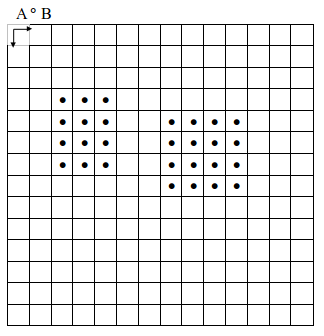
\includegraphics{q2}\\
Closing:\\
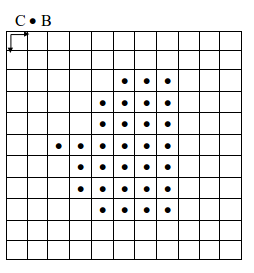
\includegraphics{q3}\\
\end{question}

\begin{question} 3
Part (a):\\
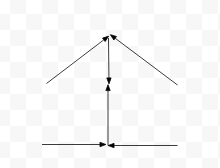
\includegraphics{q4}\\

Part (b): $$[e + \thicksim f] + \thicksim d + [a \times b]$$\\
$$[e * f] - [\thicksim e * \thicksim f]$$
\end{question}

\section{Morphology}

The pigs in this image are bright relative to everthing else in this image.
Taking that into account along with that there's a lot of grainy noise and some
text overlayed on the image, we'll probably need to do some cleaning up. The segmented
image using Otsu's method looks like this:\\

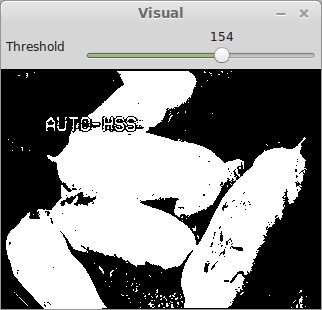
\includegraphics{binarypigs}\\

As we might suspect, there's still too much noise to see what's going on. We can
clean the bits of salt up by opening the image. I used a small cross and then a
bigger cross to clear any leftovers the first one didn't get.\\

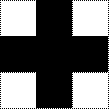
\includegraphics{cross1}
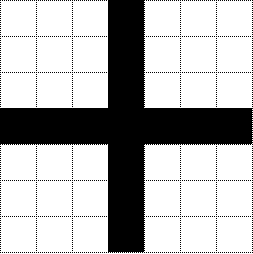
\includegraphics{cross3}\\

And then to deal with the pepper noise, I found closing the image with a square
helped better after using the cross shape.\\

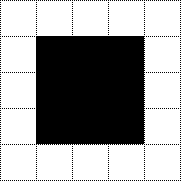
\includegraphics{square1}\\

I then filtered out the original image using the morphed binary image as a mask
to generate a nice view of just the pigs:\\

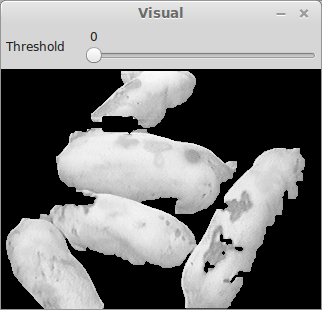
\includegraphics{morphedpigs}\\

\section{References}

\begin{enumerate}
\item OpenCV 3.0 Documentation --- http://docs.opencv.org/3.0.0/
\end{enumerate}

\end{document}